\documentclass[slidestop,mathserif]{beamer}

\usetheme{Madrid}
\usecolortheme{seahorse}

\usepackage{geometry}
\usepackage{graphicx}
\usepackage{amssymb}
\usepackage{epstopdf}
\usepackage{amsmath}  	% this permits text in eqnarray among other benefits
\usepackage{color}          	% gives color options
\usepackage{url}		% produces hyperlinks
\usepackage[english]{babel}
\usepackage[latin1]{inputenc}
\usepackage{colortbl}	% allows for color usage in tables
\usepackage{multirow}	% allows for rows that span multiple rows in tables
\usepackage{xcolor}		% this package has a variety of color options
\usepackage{calc}
\usepackage{multicol}

\setbeamertemplate{navigation symbols}{}

%User defined colors: See colors section
\xdefinecolor{oiBlue}{rgb}{0.15, 0.35, 0.55}
\xdefinecolor{gray}{rgb}{0.5, 0.5, 0.5}
\xdefinecolor{darkGray}{rgb}{0.3, 0.3, 0.3}
\xdefinecolor{darkerGray}{rgb}{0.2, 0.2, 0.2}
\xdefinecolor{rubineRed}{rgb}{0.89,0,0.30}
\xdefinecolor{linkCol}{rgb}{0.11,0.49,0.95}	
\xdefinecolor{irishGreen}{rgb}{0,0.60,0}	
\xdefinecolor{darkturquoise}{rgb}{0.44, 0.58, 0.86}
\definecolor{lightGreen}{rgb}{0.533,0.765,0.42}

\setbeamercolor*{palette primary}{fg=white,bg= oiBlue!70}
\setbeamercolor*{palette secondary}{fg=black,bg= oiBlue!20!white}
\setbeamercolor*{palette tertiary}{fg=white,bg= oiBlue!80!black!90}
\setbeamercolor*{palette quaternary}{fg=white,bg= oiBlue}

\setbeamercolor{structure}{fg= oiBlue}
\setbeamercolor{frametitle}{bg= oiBlue!70}

\setbeamercolor{disc body}{bg=oiBlue!20!white!80,fg=oiBlue!80!black!90}
\setbeamercolor{disc title}{bg=oiBlue!40!white!60,fg=oiBlue!70!black!100}


\setbeamertemplate{blocks}[shadow=false]


\newcommand{\removepagenumbers}{% 
  \setbeamertemplate{footline}{
    %
    \begin{beamercolorbox}[colsep=1.5pt]{upper separation line foot}
    \end{beamercolorbox}
    \begin{beamercolorbox}[ht=2.5ex,dp=1.125ex,%
      leftskip=.3cm,rightskip=.3cm plus1fil]{author in head/foot}%
      \leavevmode{\usebeamerfont{author in head/foot}\insertshortauthor}%
%      \hfill%
%      {\usebeamerfont{author in head/foot}\usebeamercolor[fg]{institute in head/foot}\insertshortinstitute}%
    \end{beamercolorbox}%
    \begin{beamercolorbox}[ht=2.5ex,dp=1.125ex,%
      leftskip=.3cm,rightskip=.3cm plus1fil]{title in head/foot}%
      {\usebeamerfont{title in head/foot}\insertshorttitle}%
      \hfill%
      {\usebeamerfont{author in head/foot}\usebeamercolor[fg]{institute in head/foot}\insertshortinstitute}%
    \end{beamercolorbox}%
    \begin{beamercolorbox}[colsep=1.5pt]{lower separation line foot}
    \end{beamercolorbox}
    }
} 


\newcommand{\disc}[2]{
\begin{beamerboxesrounded}[shadow = true, lower = disc body, upper = disc title]{#1}
#2
\end{beamerboxesrounded}
}


\AtBeginSection[] 
{ 
  \addtocounter{framenumber}{-1} 
  % 
  {\removepagenumbers 
    \begin{frame}<beamer> 
    \tableofcontents[currentsection] 
  \end{frame} 
  } 
} 

\usepackage{bm}

\title[JSM 2013]{GPUs, linear algebra, and efficient computing for Gaussian process models}
\author{Colin Rundel}
\date{August 6, 2013}
\institute[Duke]{Duke University}


\begin{document}

\begin{frame}[plain]
\titlepage
\end{frame}

%==================================================================================================
%==================================================================================================

\section{Background}
\addtocounter{framenumber}{-1} 

%==================================================================================================

\begin{frame}
\frametitle{The problem with GPs ...}

Unless you are lucky (or clever), Gaussian process models are difficult to scale to large problems.

\pause
\vspace{7mm}

Why?
\vspace{4mm}
\begin{itemize}
\pause \item MVN Density:

\[
  f(\bm{x}) = \frac{1}{\sqrt{(2\pi)^k|\bm{\Sigma}|}}  \exp\left(-\frac{1}{2} (\bm{x}-\bm{\mu})' \bm{\Sigma}^{-1} (\bm{x}-\bm{\mu}) \right)
\]
~\\

\pause \item Evaluating a likelihood? \pause - Invert $\Sigma$ \pause - $\mathcal{O}\left(n^3\right)$!
\vspace{2mm}
\pause \item Drawing a sample? \pause - Choleksy of $\Sigma$ \pause - $\mathcal{O}\left(n^3\right)!$
\vspace{2mm}
\pause \item Fitting a model? \pause - Update elements of $\Sigma$ \pause - $\mathcal{O}\left(n^2\right)$
\end{itemize}

\end{frame}

%%%%%%%%%%%%%%%%%%%%%%%%%%%%%%%%%%%%%%

\begin{frame}
\frametitle{What this talk is and isn't ...}

I do not have any clever solutions for these problems, but there are some very smart people out there who are working on them.

\pause\vspace{6mm}

What I do have to offer are tools to help make existing models a faster. 

\vspace{5mm}

R package, RcppGP:

\begin{itemize}
\item Low level brute force tools to improve performance (using existing GPU libraries)
\vspace{2mm}
\item High level tools for unified specification of covariance models
\vspace{2mm}
\item Painless integration with existing code
\vspace{2mm}
\item Simplify the development of new models / code
\end{itemize}

\end{frame}

%%%%%%%%%%%%%%%%%%%%%%%%%%%%%%%%%%%%%%

\begin{frame}
\frametitle{Where does RcppGP fit?}

\vfill

\begin{center}
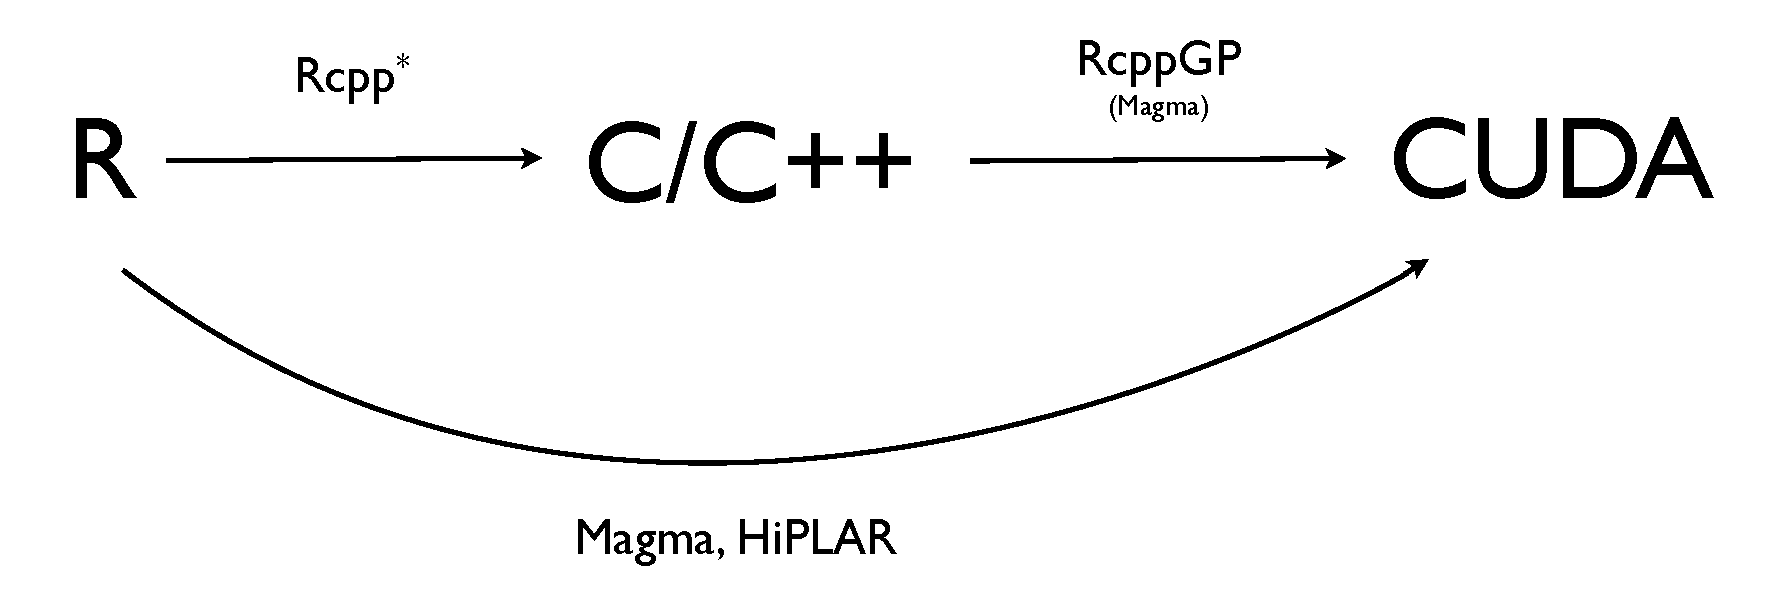
\includegraphics[width=\textwidth]{figs/diagram.pdf}
\end{center}

\vfill

\end{frame}

%%%%%%%%%%%%%%%%%%%%%%%%%%%%%%%%%%%%%%

\begin{frame}
\frametitle{Benchmarking Specs \& System}

System specs:
\begin{itemize}
\item Intel i5-2500K - 4 cores, 3.3 GHz, 16 GB
\item GeForce GTX 460 - 336 cores, 1.44 GHz, 1024 MB
\end{itemize}

\vspace{5mm}

Software specs:
\begin{itemize}
\item Ubuntu 13.04
\item OpenBlas 0.2.6
\item CUDA 5.5 RC1
\item Magma 1.4 beta1
\item Armadillo 3.900.0 
\end{itemize}

\vspace{5mm}

All performance metrics reflect pure C++ implementations (CPU) versus C++ / CUDA / Magma implementations (GPU).

\end{frame}

%%%%%%%%%%%%%%%%%%%%%%%%%%%%%%%%%%%%%%

\begin{frame}
\frametitle{Performance - Calculating covariance matrix}

\begin{center}
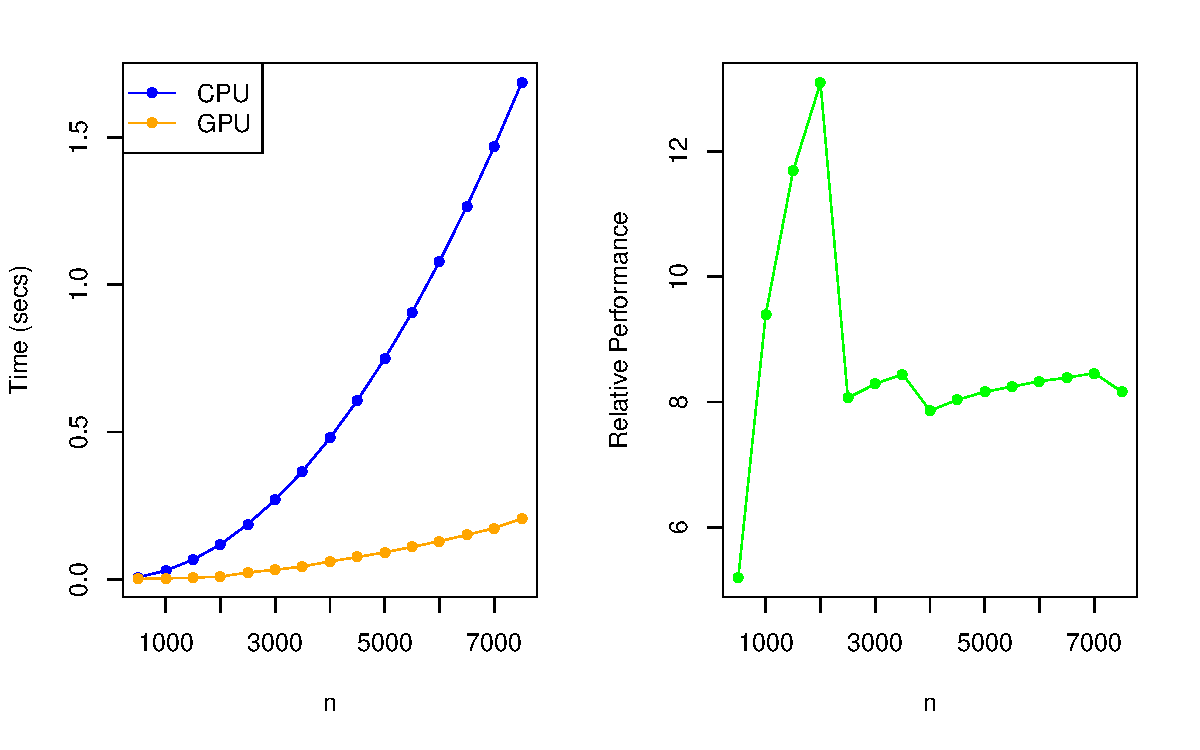
\includegraphics[width=\textwidth]{figs/cov_bench.pdf}
\end{center}

\end{frame}

%%%%%%%%%%%%%%%%%%%%%%%%%%%%%%%%%%%%%%

\begin{frame}
\frametitle{Performance - Cholesky decomposition}

\begin{center}
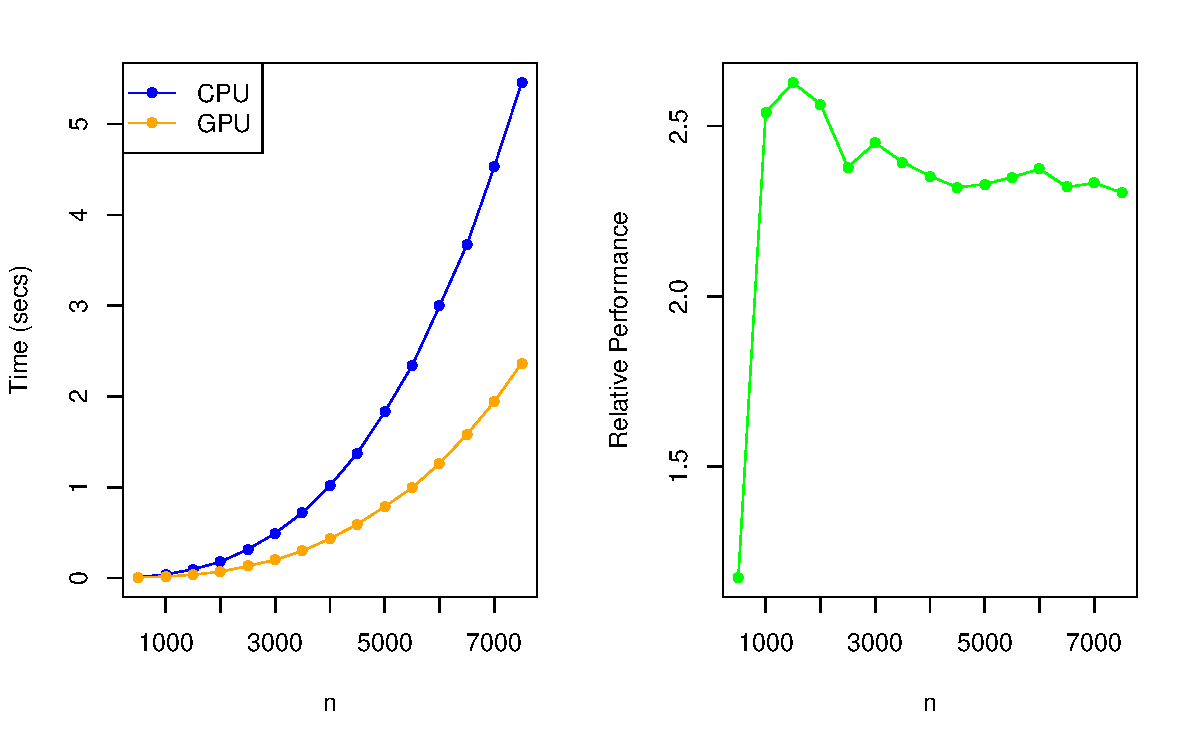
\includegraphics[width=\textwidth]{figs/chol_cov_bench.pdf}
\end{center}

\end{frame}

%%%%%%%%%%%%%%%%%%%%%%%%%%%%%%%%%%%%%%

\begin{frame}
\frametitle{Performance - Inverse covariance matrix}

\begin{center}
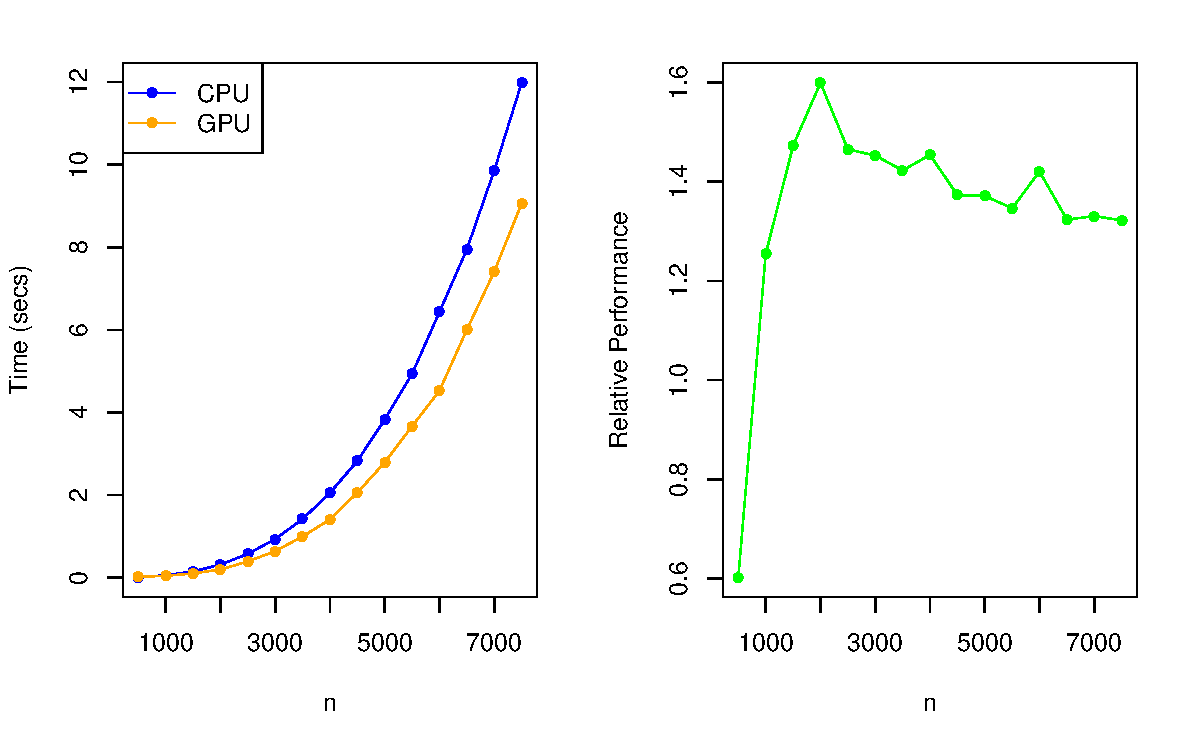
\includegraphics[width=\textwidth]{figs/inv_cov_bench.pdf}
\end{center}

\end{frame}

%%%%%%%%%%%%%%%%%%%%%%%%%%%%%%%%%%%%%%

\begin{frame}
\frametitle{Putting RcppGP to use}

spBayes is a fantastic package for fitting Bayesian spatial models, but

\vspace{4mm}

\begin{itemize}
\item wanted expanded functionality, in particular

\begin{itemize}
\item arbitrary coordinate dimensions
\item more flexible covariance models
\item inspired by GPStuff
\end{itemize}

\item improve performance wherever possible.
\end{itemize}

\pause
\vspace{5mm}
What to do?

\pause

\begin{itemize}
\item Rewrote spLM and spPredict using Rcpp and RcppArmadillo.
\vspace{2mm}
\item Modified the rewrite to use GPU using RcppGP.
\end{itemize}
\end{frame}

%%%%%%%%%%%%%%%%%%%%%%%%%%%%%%%%%%%%%%

\begin{frame}
\frametitle{CPU vs GPU Code}

\begin{center}
\vspace{-5mm}
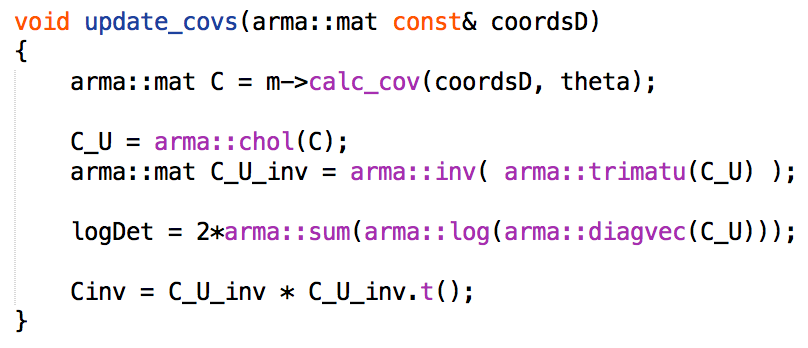
\includegraphics[width=0.7\textwidth]{figs/cpu_cov.png}

\vspace{5mm}

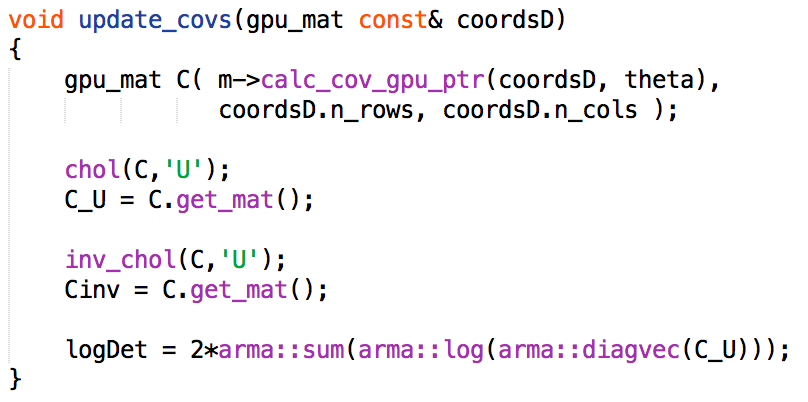
\includegraphics[width=0.7\textwidth]{figs/gpu_cov.png}
\end{center}
\end{frame}

%%%%%%%%%%%%%%%%%%%%%%%%%%%%%%%%%%%%%%

\begin{frame}
\frametitle{Example - Leaf Area Index}

\vspace{-7mm}
\begin{center}
\only<1-3>{ 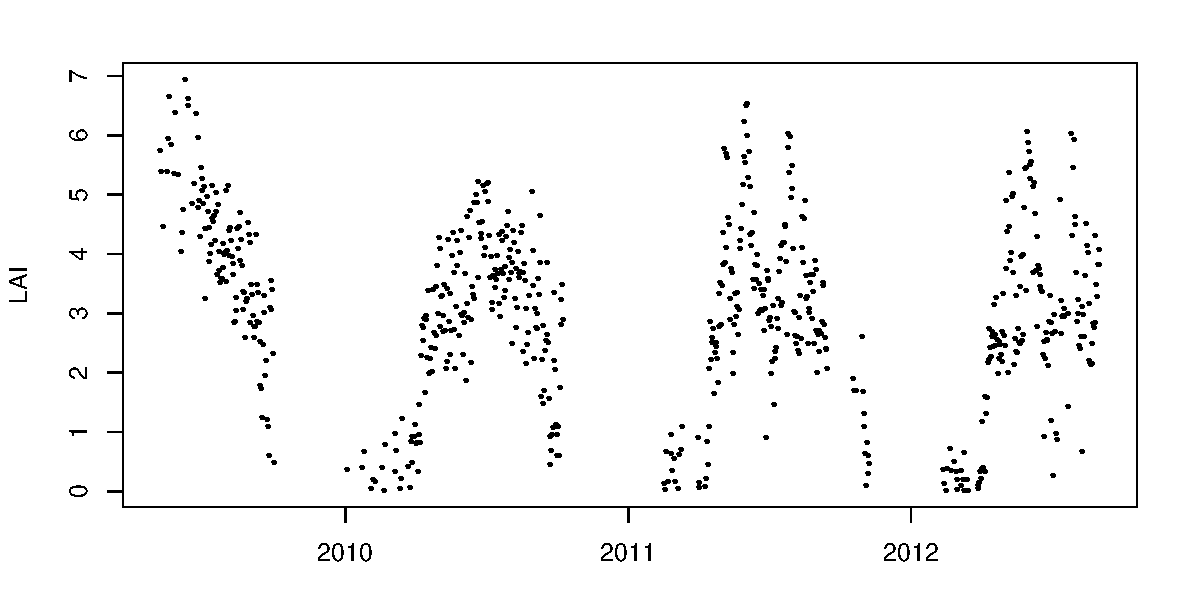
\includegraphics[width=\textwidth]{figs/LAI.pdf} }
\only<4>{ 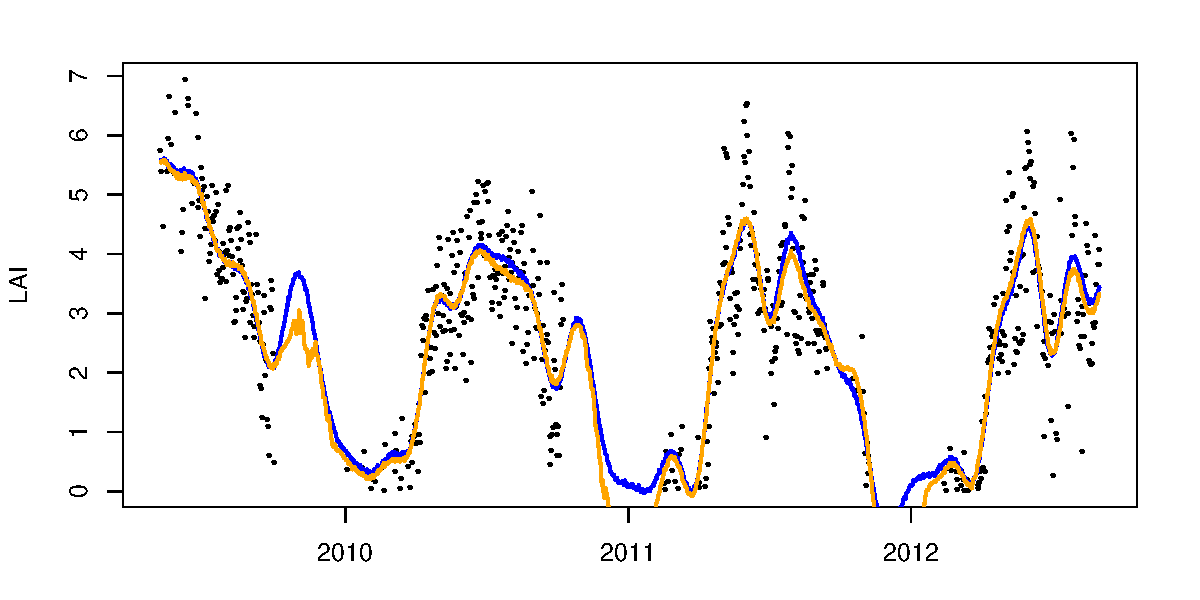
\includegraphics[width=\textwidth]{figs/LAI_pred.pdf} }
\end{center}

\vspace{-5mm}

%\only<2->{
%\[C(x,x') = \tau^2 \mathit{I} + \sigma^2 \exp\left( -\frac{1}{2}\left(\frac{\lVert x-x' \rVert}{1/\phi}\right)^2-\frac{2\%sin^2\left(\frac{1}{2}\frac{\lVert x-x' \rVert}{\gamma}\right)}{1/\lambda^2} \right)\]
%}

\begin{center}
\only<2>{  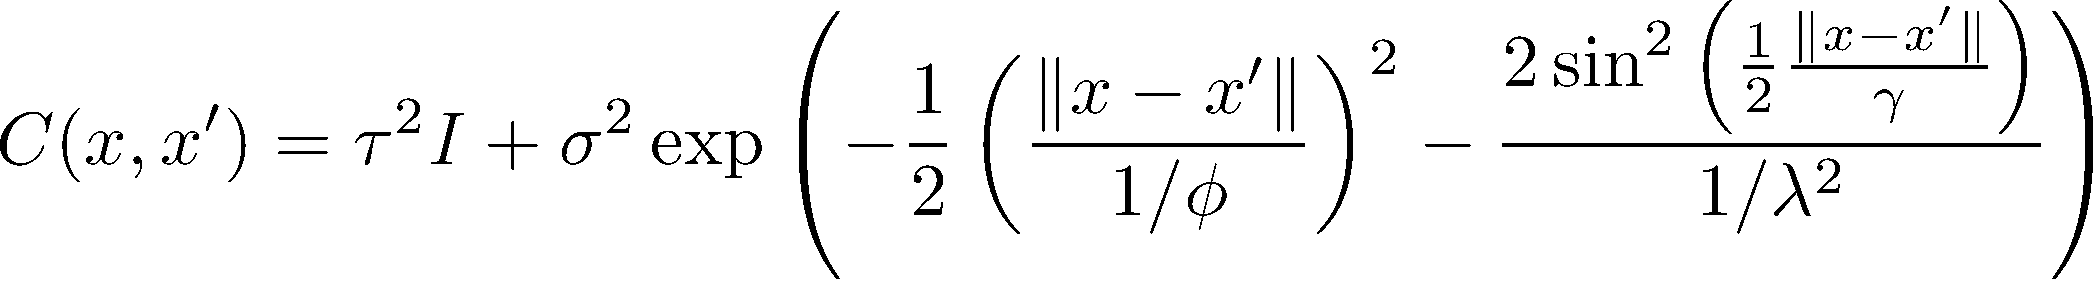
\includegraphics[width=0.8\textwidth]{figs/cov_eq.pdf} }
\only<3->{ 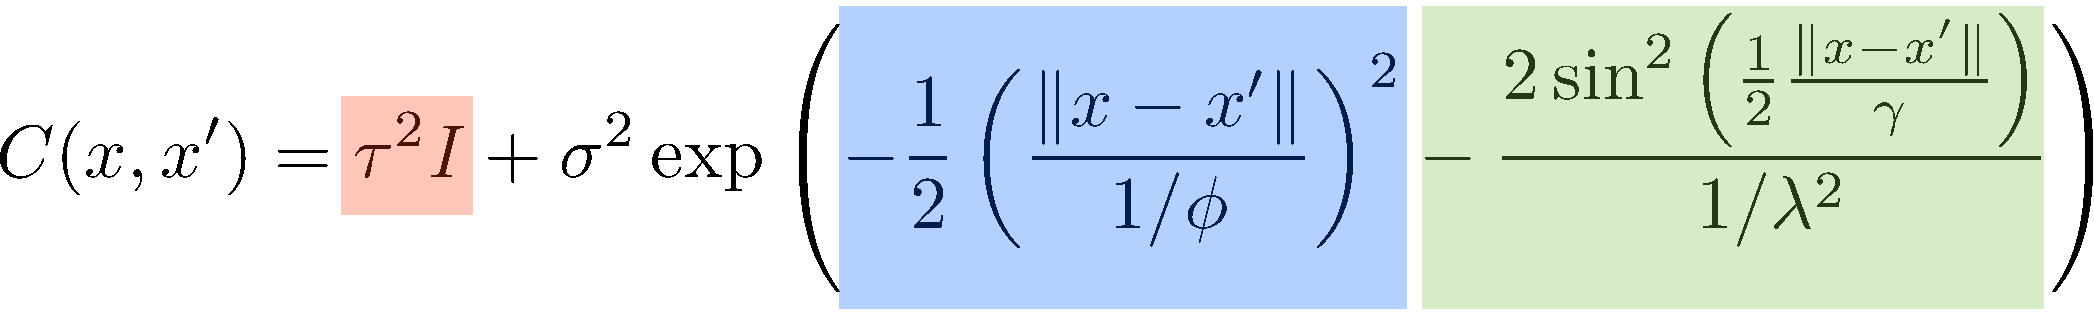
\includegraphics[width=0.8\textwidth]{figs/cov_eq2.pdf} }
\end{center}

\end{frame}

%%%%%%%%%%%%%%%%%%%%%%%%%%%%%%%%%%%%%%

\begin{frame}
\frametitle{Covariance models}

\vspace{-5mm}

\begin{center}
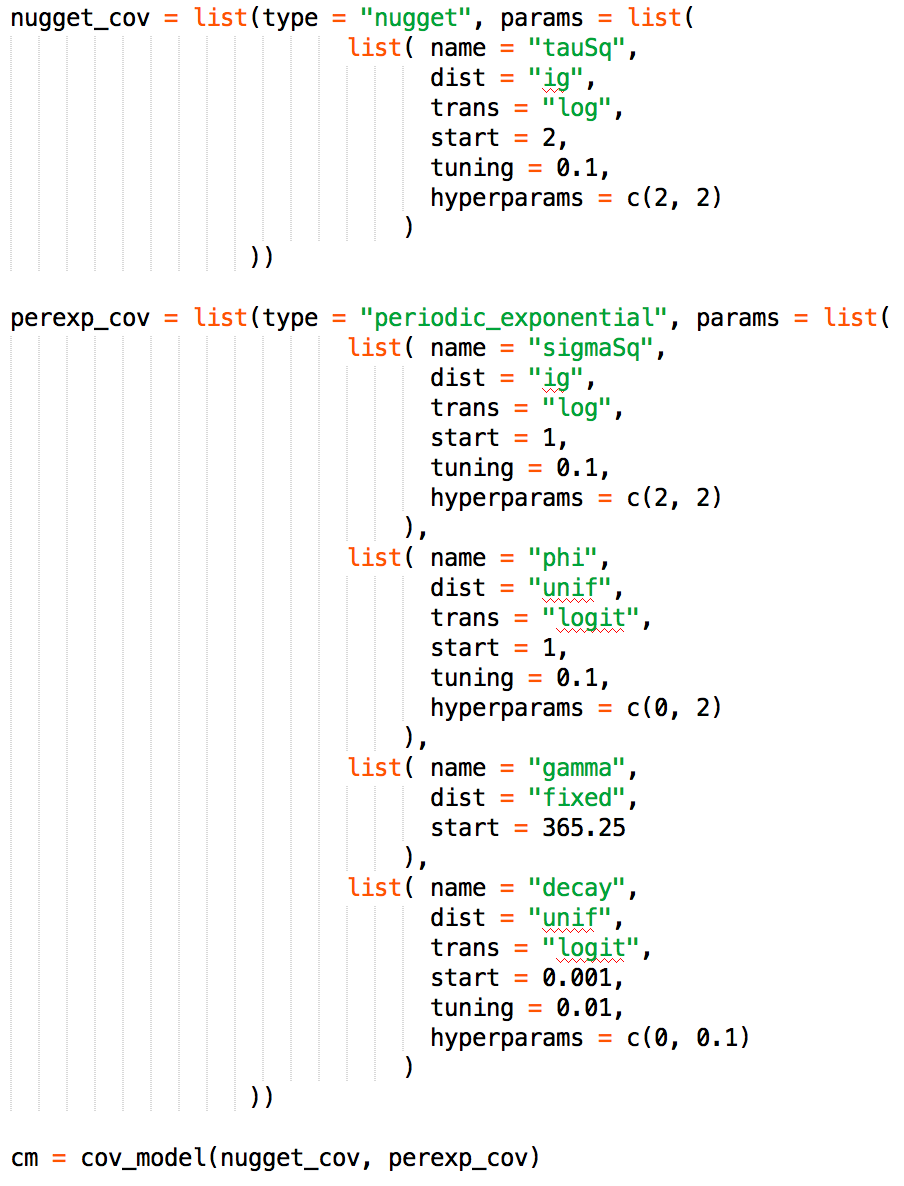
\includegraphics[width=0.5\textwidth]{figs/cov_model.png}
\end{center}

\end{frame}

%%%%%%%%%%%%%%%%%%%%%%%%%%%%%%%%%%%%%%

\begin{frame}
\frametitle{Example - Leaf Area Index - Results}

Model Fitting: 
\vspace{-2mm}
\begin{center}
$n = 700$, $\#_{iter} = 5000$

\vspace{4mm}

\begin{tabular}{c|cc|c}
    & Run time (sec) & sec / iter & Rel. Performance \\
\hline
CPU & 491.8          & 0.0983     & 3.55 \\
GPU & 138.5          & 0.0277     & 1.00 \\
\hline
\end{tabular}
\end{center}

\vspace{7mm}

Model Prediction: 
\vspace{-2mm}
\begin{center}
$n = 1212$, $\#_{pred} = 1000$

\vspace{4mm}

\begin{tabular}{c|cc|c}
    & Run time (sec) & sec / iter & Rel. Performance \\
\hline
CPU & 459.5          & 0.460      & 5.15 \\
GPU &  89.2          & 0.089      & 1.00 \\
\hline
\end{tabular}
\end{center}

\end{frame}

%%%%%%%%%%%%%%%%%%%%%%%%%%%%%%%%%%%%%%

\begin{frame}
\frametitle{Summary}

\begin{enumerate}
\item Goal is to make GPU computing available and painless for common bottlenecks
\item Use of GPU only for covariance calculations and common decompositions can result in a 3-5x speedup
\item High level functionality makes common tasks in GP models easier
\item Core tools are methodology agnostic
\item 12 minutes is not enough time to get into details, look at the code (particularly spPredict)
\end{enumerate}

\vspace{5mm} \pause

Coming soon:
\begin{enumerate}
\item Stabilization of interface
\item Compatibility with RcppAttributes
\item Full support for GPP and mGPP in spLM example
\item Documentation
\end{enumerate}

\end{frame}

%%%%%%%%%%%%%%%%%%%%%%%%%%%%%%%%%%%%%%

\begin{frame}
\frametitle{Questions, Comments?}
\vfill
\begin{center}
{\Large
\renewcommand*\arraystretch{1.5}
\begin{tabular}{lll}
Email        & : & rundel@gmail.com \\
RcppGP       & : & {\normalsize \urlwofont{http://github.com/rundel/RcppGP}} \\
Presentation & : & {\normalsize \urlwofont{http://github.com/rundel/Presentations/}} \\
\end{tabular}
}
\end{center}
\vfill
\end{frame}

\end{document}